\begin{figure}[ht]
\centering
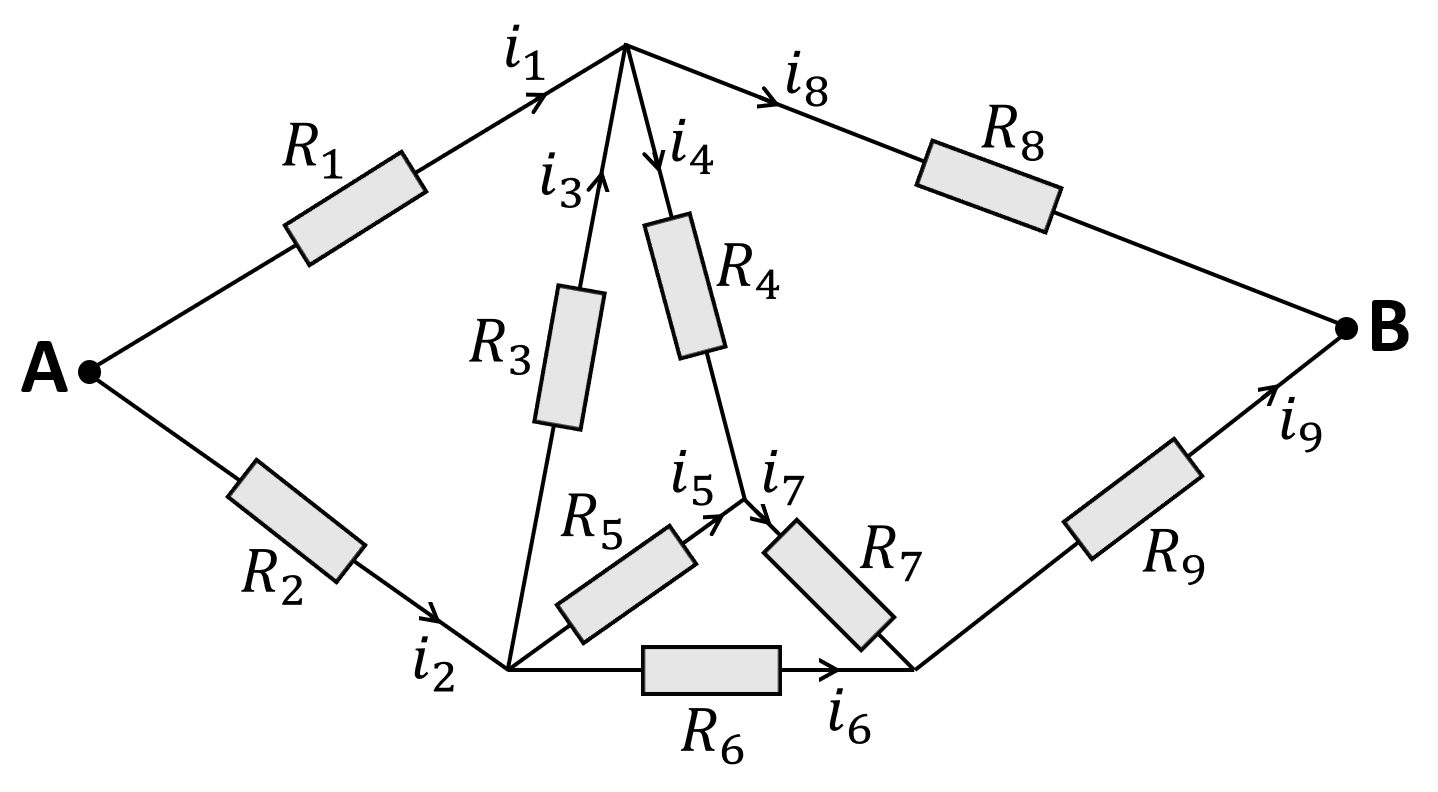
\includegraphics[width=0.6\textwidth,keepaspectratio]{Problem_2/Figs/P2A.png}
\end{figure}

Xét một mạch điện cấu tạo từ các điện trở $R_1$, $R_2$, ..., $R_8$, $R_9$. Khi đặt hiệu điện thế $1V$ vào hai đầu mạch A và B thì thu được phân bố dòng điện với chiều đi như hình vẽ, cường độ đo được theo đơn vị $mA$ là:
\begin{equation}
i_1 = 33 \ , \ i_2 = 28 \ , \ i_3 = 5 \ , \ i_4 = 2 \ , \ i_5 = 7 \ , \ i_6 = 16 \ , \ i_7 = 9 \ , \ i_8 = 36 \ , \ i_9 = 25 \ . \nonumber
\end{equation}
Với những thông tin đã cho thì liệu có thể xác định được giá trị của các điện trở hay không, và nếu có thì hãy xác định $R_1$ và $R_9$.